% ---------------------------------------------------------------------
% -------------- PREAMBLE ---------------------------------------------
% ---------------------------------------------------------------------
\documentclass[12pt,a4paper,finnish,oneside]{article}
%\documentclass[12pt,a4paper,finnish,twoside]{article}
%\documentclass[12pt,a4paper,finnish,oneside,draft]{article} % luonnos, nopeampi

% Valitse 'input encoding':
%\usepackage[latin1]{inputenc} % merkistökoodaus, jos ISO-LATIN-1:tä.
\usepackage[utf8]{inputenc}   % merkistökoodaus, jos käytetään UTF8:a
% Valitse 'output/font encoding':
%\usepackage[T1]{fontenc}      % korjaa ääkkösten tavutusta, bittikarttana
\usepackage{ae,aecompl}       % ed. lis. vektorigrafiikkana bittikartan sijasta
% Kieli- ja tavutuspaketit:
\usepackage[english,swedish,finnish]{babel}
% Kurssin omat asetukset aaltosci_t.sty:
\usepackage{aaltosci_t}
% Jos kirjoitat muulla kuin suomen kielellä valitse:
%\usepackage[finnish]{aaltosci_t}           
%\usepackage[swedish]{aaltosci_t}           
%\usepackage[english]{aaltosci_t}           
% Muita paketteja:
\usepackage{alltt}
\usepackage{amsmath}   % matematiikkaa
\usepackage{calc}      % käytetään laskurien (counter) yhteydessä (tiedot.tex)
\usepackage{eurosym}   % eurosymboli: \euro{}
\usepackage{url}       % \url{...}
\usepackage{listings}  % koodilistausten lisääminen
\usepackage{algorithm} % algoritmien lisääminen kelluvina
\usepackage{algorithmic} % algoritmilistaus
\usepackage{hyphenat}  % tavutuksen viilaamiseen liittyvä (hyphenpenalty,...)
\usepackage{supertabular,array}  % useampisivuinen taulukko

% Koko dokumentin kattavia asetuksia:

% Tavutettavia sanoja:
%\hyphenation{vää-rin me-ne-vi-en eri-kois-ten sa-no-jen tavu-raja-ehdo-tuk-set}
% Huomaa, että ylläoleva etsii tarkalleen kyseisiä merkkijonoja, eikä
% ymmärrä taivutuksia. Paikallisesti tekstin seassa voi myös ta\-vut\-taa.

% Rangaistaan tavutusta (ei toimi?! Onko hyphenat-paketti asennettu?)
\hyphenpenalty=10000   % rangaistaan tavutuksesta, 10000=ääretön
\tolerance=1000        % siedetään välejä riveillä
% titlesec-paketti auttaa, jos tämän mukana menee sekaisin

% Tekstiviitteiden ulkoasu.
% Pakettiin natbib.sty/aaltosci.bst liittyen katso esim. 
% http://merkel.zoneo.net/Latex/natbib.php
% jossa selitykset citep, citet, bibpunct, jne.
% Valitse alla olevista tai muokkaa:
\bibpunct{(}{)}{;}{a}{,}{,}    % a = tekijä-vuosi (author-year)
%\bibpunct{[}{]}{;}{n}{,}{,}    % n = numero [1],[2] (numerical style)

% Rivivälin muuttaminen:
\linespread{1.24}\selectfont               % riviväli 1.5
%\linespread{1.24}\selectfont               % riviväli 1, kun kommentoit pois

% ---------------------------------------------------------------------
% -------------- DOCUMENT ---------------------------------------------
% ---------------------------------------------------------------------

\begin{document}

% -------------- Tähän dokumenttiin liittyviä valintoja  --------------

%\raggedright         % Tasattu vain vasemmalta, ei tavutusta
% ----------------- joitakin makroja ----------------------------------
%
% \newcommand{\sinunKomentosi}[argumenttienMäärä]{komennot%
% voiJakaaRiveille%
% jaArgumenttienViittaus#1,#2,#argumenttienMäärä}

% Joskus voi olla tarpeen kommentoida jotakin. Ei suositella. 
% Äläkä unohda lopulliseen! 
\newcommand{\Kommentti}[1]{\fbox{\textbf{OMA KOMMENTTI:} #1}}
% Käyttö: Kilometri on 1024 metriä. \Kommentti{varmista tämä vielä}.
% Eli newcommand:n komentosanan jälkeen hakasaluissa argumenttien lkm,
%  ja argumentteihin viitataa #1, #2, ...

%  Comment out this \DRAFT macro if this version no longer is one!  XXX
%\newcommand{\DRAFT}{\begin{center} {\it DRAFT! \hfill --- \hfill DRAFT!
%\hfill --- \hfill DRAFT! \hfill --- \hfill DRAFT!}\end{center}}

%  Use this \DRAFT macro in the final version - or comment out the 
%  draft-command
% \newcommand{\DRAFT}{~}

% %%%%%%%% MATEMATIIKKA %%%%%%%%%%%%%%%%%

% Määrätty integraali
\newcommand{\myInt}[4]{%
\int_{#1}^{#2} #3 \, \textrm{d}{#4}}

% http://kapsi.fi/jks/satfaq/
%\newcommand{\vii}{\mathop{\Big/}}
%\newcommand{\viiva}[2]{\vii\limits_{\!\!\!\!{#1}}^{\>\,{#2}}}
%%\[ \intop_0^{10} \frac{x}{x^2+1} \,\mathrm{d}x
%%= \viiva{0}{10} \frac{1}{2}\ln(x^2+1) \]

% matht.sty, Simo K. Kivelä, 01.01.2002, 07.04.2004, 19.11.2004, 21.02.2005
% Kokoelma matemaattisten lausekkeiden kirjoittamista helpottavia
% määrittelyjä.

% 07.04.2004 Muutama lisäys ja muutos tehty: \ii, \ee, \dd, \der,
% \norm, \abs, \tr.
%
% 19.11.2004 Korjattu määrittelyjä: \re, \im, \norm;
% lisätty \trp (transponointi), \hrm (hermitointi), \itgr (rakenteellinen
% integraali), ympäristö Cmatrix (hakasulkumatriisi);
% vanha transponointi \tr on mukana edelleen, mutta ei suositella.

% Pakotettu rivinvaihto, joka voidaan tarvittaessa määritellä
% uudelleen: 

%\newcommand{\nl}{\newline}

% Logiikan symboleja (<=> ja =>) hieman muunnettuina:

%\newcommand{\ifftmp}{\;\Leftrightarrow\;}
%\newcommand{\impltmp}{\DOTSB\;\Rightarrow\;}

% 'siten, että' -lyhenne ja hattupääyhtäläisyysmerkki vastaavuuden
% osoittamiseen: 

%\newcommand{\se}{\quad \text{siten, että} \quad}
%\newcommand{\vs}{\ {\widehat =}\ }

% Lukujoukkosymbolit:

%\newcommand{\N}{\ensuremath{\mathbb N}}
%\newcommand{\Z}{\ensuremath{\mathbb Z}}
%\newcommand{\Q}{\ensuremath{\mathbb Q}}
%\newcommand{\R}{\ensuremath{\mathbb R}}
%\newcommand{\C}{\ensuremath{\mathbb C}}

% Reaali- ja imaginaariosa, imaginaariyksikkö:

%\newcommand{\re}{\operatorname{Re}}
%\newcommand{\im}{\operatorname{Im}}
%\newcommand{\ii}{\mathrm{i}}

% Differentiaalin d, Neperin luku:

%\newcommand{\dd}{\mathrm{d}}
%\newcommand{\ee}{\mathrm{e}}

% Vektorimerkintä, joka voidaan tarvittaessa määritellä uudelleen
% (tämä tekee vektorit lihavoituina):

%\newcommand{\V}[1]{{\mathbf #1}}

% Kulmasymboli:

%\renewcommand{\angle}{\sphericalangle}

% Vektorimerkintä, jossa päälle pannaan iso nuoli;
% esimerkiksi \overrightarrow{AB} (tämmöisiä olemassaolevien
% symbolien uudelleenmäärittelyjä ei kyllä pitäisi tehdä):

%\renewcommand{\vec}[1]{\overrightarrow{#1}}

% Vektoreiden vastakkaissuuntaisuus:

%\newcommand{\updownarrows}{\uparrow\negthinspace\downarrow}

% Itseisarvot ja normi:

%\newcommand{\abs}[1]{{\left\vert#1\right\vert}}
%\newcommand{\norm}[1]{{\left\Vert #1 \right\Vert}}

% Transponointi ja hermitointi:

%\newcommand{\trp}[1]{{#1}\sp{\operatorname{T}}}
%\newcommand{\hrm}[1]{{#1}\sp{\operatorname{H}}}

% Vanha transponointi; jäljellä yhteensopivuussyistä, ei syytä käyttää.
%\newcommand{\tr}{{}^{\text T}}

% Arcus- ja area-funktiot, jossa päähaara osoitetaan nimen päälle
% vedetyllä vaakasuoralla viivalla (alkaa olla vanhentunutta,
% voitaisiin luopua):

%\newcommand{\arccot}{\operatorname{arccot}}
%\newcommand{\asin}{\operatorname{\overline{arc}sin}}
%\newcommand{\acos}{\operatorname{\overline{arc}cos}}
%\newcommand{\atan}{\operatorname{\overline{arc}tan}}
%\newcommand{\acot}{\operatorname{\overline{arc}cot}}

%\newcommand{\arsinh}{\operatorname{arsinh}}
%\newcommand{\arcosh}{\operatorname{arcosh}}
%\newcommand{\artanh}{\operatorname{artanh}}
%\newcommand{\arcoth}{\operatorname{arcoth}}
%\newcommand{\acosh}{\operatorname{\overline{ar}cosh}}

% Signum, syt, pyj:

%\newcommand{\sg}{\operatorname{sgn}}
%\renewcommand{\gcd}{\operatorname{syt}}
%\newcommand{\lcm}{\operatorname{pyj}}

% Lyhennemerkintöjä: derivaatta, osittaisderivaatta, gradientti,
% derivaattaoperaattori, vektorin komponentti, integraalin ylä- ja
% alasumma, Suomessa (ja Saksassa?) käytetty integraalin sijoitus-
% merkintä, integraali (rakenteellinen määrittely):

%\newcommand{\der}[2]{\frac{\dd #1}{\dd #2}}
%\newcommand{\osder}[2]{\frac{\partial #1}{\partial #2}}
%\newcommand{\grad}{\operatorname{grad}}
%\newcommand{\Df}{\operatorname{D}} 
%\newcommand{\comp}{\operatorname{comp}}
%\newcommand{\ys}[1]{\overline S_{#1}}
%\newcommand{\as}[1]{\underline S_{#1}}
%\newcommand{\sijoitus}[2]{\biggl/_{\null\hskip-6pt #1}^{\null\hskip2pt #2}} 
%\newcommand{\itgr}[4]{\int_{#1}^{#2}#3\,\dd #4}

% Matriiseja, joille voidaan antaa alkioiden sijoittamista sarakkeen
% vasempaan tai oikeaan reunaan tai keskelle osoittava lisäparametri
% (l, r tai c); ympärillä kaarisulut, hakasulut, pystyviivat (determinantti)
% tai ei mitään;
% esimerkiksi \begin{cmatrix}{ll}1 & -1 \\ -1 & 1 \end{cmatrix}:

%\newenvironment{cmatrix}[1]{\left(\begin{array}{#1}}{\end{array}\right)}
%\newenvironment{Cmatrix}[1]{\left[\begin{array}{#1}}{\end{array}\right]}
%\newenvironment{dmatrix}[1]{\left|\begin{array}{#1}}{\end{array}\right|}
%\newenvironment{ematrix}[1]{\begin{array}{#1}}{\end{array}}

% Kaunokirjoitussymboli:

%\newcommand{\Cal}{\mathcal}

% Isokokoinen summa:

%\newcommand{\dsum}[2]{{\displaystyle \sum_{#1}^{#2}}}

% Tuplaintegraali umpinaisen pinnan yli; korvataan jos parempi löytyy:
%\newcommand\oiint{\begingroup
% \displaystyle \unitlength 1pt
% \int\mkern-7.2mu
% \begin{picture}(0,3)
%   \put(0,3){\oval(10,8)}
% \end{picture}
% \mkern-7mu\int\endgroup}
       % Haetaan joitakin makroja

% Kieli:
% Kielesi, jolla kandidaatintyön kirjoitat: finnish, swedish, english.
% Tästä tulee mm. tietyt otsikkonimet ja kuva- ja taulukkoteksteihin 
% (Kuva, Figur, Figure), (Taulukko, Tabell, Table) sekä oikea tavutus.
\selectlanguage{finnish}
%\selectlanguage{swedish}
%\selectlanguage{english}

% Sivunumeroinnin kanssa pieniä ristiriitaisuuksia.
% Toimitaan pääosin lähteen "Kirjoitusopas" luvun 5.2.2 mukaisesti.
% Sivut numeroidaan juoksevasti arabialaisin siten että 
% ensimmäiseltä nimiölehdeltä puuttuu numerointi.
\pagestyle{plain}
\pagenumbering{arabic}
% Muita tapoja: kandiohjeet: ei numerointia lainkaan ennen tekstiosaa
%\pagestyle{empty}
% Muita tapoja: kandiohjeet: roomalainen numerointi alussa ennen tekstiosaa
%\pagestyle{plain}
%\pagenumbering{roman}        % i,ii,iii, samalla alustaa laskurin ykköseksi

% ---------------------------------------------------------------------
% -------------- Luettelosivut alkavat --------------------------------
% ---------------------------------------------------------------------

% -------------- Nimiölehti ja sen tiedot -----------------------------
%
% Nimiölehti ja tiivistelmä kirjoitetaan seminaarin mukaan joko
% suomeksi tai ruotsiksi (ellei erityisesti kielenä ole englanti). 
% Tiivistelmän voi suomen/ruotsin lisäksi kirjoittaa halutessaan
% myös englanniksi. Eli tiivistelmiä tulee yksi tai kaksi kpl.
%
% "\MUUTTUJA"-kohdat luetaan aaltosci_t.sty:ä varten.

\author{Teemu Teekkari}

% Otsikko nimiölehdelle. Yleensä sama kuin seuraavana oleva \TITLE, 
% mutta jos nimiölehdellä tarvetta "kaksiosaiselle" kaksiriviselle
\title{\LaTeX{}-pohja kandidaatintyötä varten ohjeiden kera ja varuilta %
kokeillaan vähän ylipitkää otsikkoa}
% 2-osainen otsikko:
%\title{\LaTeX{}-pohja kandidaatintyölle \\[5mm] Pitkiä rivejä kokeilun vuoksi.}

% Otsikko tiivistelmään. Jos lisäksi engl. tiivistelmä, niin viimeisin:
\TITLE{\LaTeX{}-pohja kandidaatintyötä varten ohjeiden kera ja varuilta %
kokeillaan vähän ylipitkää otsikkoa}
%\TITLE{\LaTeX{} för kandidatseminariet med jättelång rubrik som fortsätter och
% fortsätter ännu}
\ENTITLE{\LaTeX{} template for Bachelor thesis with a pretty long title %
line which continues ynd continues}
% 2-osainen otsikko korvataan täällä esim. pisteellä:
%\TITLE{\LaTeX{}-pohja kandidaatintyölle. Pitkiä rivejä kokeilun vuoksi.}

% Ohjaajan laitos suomi/ruotsi ja tarvittaessa eng (tiivistelmän kieli/kielet)
\DEPT{Poimi tähän ohjaajasi laitos, DEPT, main.tex}
% suomi:
%\DEPT{Tietotekniikan laitos}               % T
%\DEPT{Tietojenkäsittelytieteen laitos}     % TKT
%\DEPT{Mediatekniikan laitos}               % ME
% ruotsi:
%\DEPT{Institutionen för datateknik}        % T
%\DEPT{Institutionen för datavetenskap}     % TKT
%\DEPT{Institutionen för mediateknik}       % ME
% englanti:
%\ENDEPT{Department of Computer Science Engineering}     % T
%\ENDEPT{Department of Information and Computer Science} % TKT
%\ENDEPT{Department of Media Technology}                 % ME

% Vuosi ja päivämäärä, jolloin työ on jätetty tarkistettavaksi.
\YEAR{2011}
\DATE{28. marraskuuta 2011}
%\DATE{31. helmikuuta 2011}
%\DATE{Den 31 februari 2011}
\ENDATE{February 31, 2011}

% Kurssin vastuuopettaja ja työsi ohjaaja(t)
\SUPERVISOR{Ma professori Tomi Janhunen}
\INSTRUCTOR{Ohjaajantitteli Sinun Ohjaajasi}
%\INSTRUCTOR{Ohjaajantitteli Sinun Ohjaajasi, ToinenTitt Matti Meikäläinen}
% DI       // på svenska DI diplomingenjör
% TkL      // TkL teknologie licentiat
% TkT      // TkD teknologie doctor
% Dosentti Dos. // Doc. Docent
% Professori Prof. // Prof. Professor
% 
% Jos tiivistelmä englanniksi, niin:
\ENSUPERVISOR{Professor (pro tem) Tomi Janhunen}
\ENINSTRUCTOR{Your instructor, titleOfInstructor}
% M.Sc. (Tech)  // M.Sc. (Eng)
% Lic.Sc. (Tech)
% D.Sc. (Tech)   // FT filosofian tohtori, PhD Doctor of Philosophy
% Docent
% Professor

% Kirjoita tänne HOPS:ssa vahvistettu pääaineesi.
% Pääainekoodit TIK-opinto-oppaasta.

\PAAAINE{Tähän sinun pääaineesi nimi, kts main.tex}
\CODE{Txxxx tai ILyyyy}

%\PAAAINE{Ohjelmistotuotanto ja -liiketoiminta}
%\CODE{T3003}
%
%\PAAAINE{Tietoliikenneohjelmistot}
%\CODE{T3005}
%
%\PAAAINE{WWW-teknologiat} % vuodesta 2010
%\CODE{IL3012}
%
%\PAAAINE{Mediatekniikka} % vuoteen 2010, kts. seur.
%\CODE{T3004}
%
%\PAAAINE{Mediatekniikka} % vuodesta 2010, kts. edell.
%\CODE{IL3011}
%
%\PAAAINE{Tietojenkäsittelytiede} % vuodesta 2010
%\CODE{IL3010}
%
%\PAAAINE{Informaatiotekniikka} % vuoteen 2010
%\CODE{T3006}
%
%\PAAAINE{Tietojenkäsittelyteoria} % vuoteen 2010
%\CODE{T3002}
%
%\PAAAINE{Ohjelmistotekniikka}
%\CODE{T3001}

% Avainsanat tiivistelmään. Tarvittaessa myös englanniksi:

\KEYWORDS{avain, sanoja, niitäkin, tähän, vielä, useampi, vaikkei, %
niitä, niin, montaa, oikeasti, tarvitse}
\ENKEYWORDS{key, words, the same as in FIN/SWE}

% Tiivistelmään tulee opinnäytteen sivumäärä.
% Kirjoita lopulliset sivumäärät käsin tai kokeile koodia. 
%
% Ohje 29.8.2011 kirjaston henkilökunnalta:
%   - yhteissivumäärä nimiölehdeltä ihan loppuun
%   - "kaikkien yksinkertaisin ja yksiselitteisin tapa"
%
% VANHA // Ohje 14.11.2006, luku 4.2.5:
% VANHA // - sivumäärä = tekstiosan (alkaen johdantoluvusta) ja 
% VANHA //  lähdeluettelon sivumäärä, esim. "20"
% VANHA // - jos liitteet, niin edellisen lisäksi liitteiden sivumäärä,
% VANHA //  tyyli "20 + 5", jossa 5 sivua liitteitä 
% VANHA // - HUOM! Tässä oletuksena sivunumerointi alkaa nimiölehdestä 
% VANHA //  sivunumerolla 1. %   Toisin sanoen, viimeisen lähdeluettelosivun 
% VANHA //  sivunumero EI ole sivujen määrä vaan se pitää laskea tähän käsin

\PAGES{Kirjoita tähän oikea määrä, tässä esimerkissä 23}
%\PAGES{23}  % kaikki sivut laskettuna nimiölehdestä lähdeluettelon tai 
             % mahdollisten liitteiden loppuun. Tässä 23 sivua

%\thispagestyle{empty}  % nimiölehdellä ei ole sivunumerointia; tyylin mukaan ei tehdäkään?!

\maketitle             % tehdään nimiölehti

% -------------- Tiivistelmä / abstract -------------------------------
% Lisää abstrakti kandikielellä (ja halutessasi lisäksi englanniksi).

% Edelleen sivunumerointiin. Eräs ohje käskee aloittaa sivunumeroiden
% laskemisen nimiösivulta kuitenkin niin, että sille ei numeroa merkitä
% (Kauranen, luku 5.2.2). Näin ollen ensimmäisen tiivistelmän sivunumero
% on 2. \maketitle komento jotenkin kadottaa sivunumeronsa.
\setcounter{page}{2}    % sivunumeroksi tulee 2

% Tiivistelmät tehdään viimeiseksi. 
%
% Tiivistelmä kirjoitetaan käytetyllä kielellä (JOKO suomi TAI ruotsi)
% ja HALUTESSASI myös samansisältöisenä englanniksi.
%
% Avainsanojen lista pitää merkitä main.tex-tiedoston kohtaan \KEYWORDS.

\begin{fiabstract}
Tämä kandinaatintyö käsittelee eleentunnistusta Kinect-sensorilla.
Työssä esitellään yleisesti eleentunnistusongelmaa ja miten Kinectin 3D-videokuva vastaa eleentunnistuksen haasteisiin.
Työssä tutustutaan ChaLearn Gesture Challenge -kilpailun kilpailutöihin ja sitä kautta alan uusimpaan tutkimukseen.

Työssä havaitaan, että eleentunnistuksen suurimpia haasteita on luokkien sisäinen varianssi. Sama ele näyttää erilaiselta
esittäjästä ja tilanteesta riippuen. Syvyyskuva kuitenkin pienentää tekstuureista ja värityksestä johtuvaa varianssia.
Syvyyskuvan avulla voidaan luotettavasti erottaa myös ihmishahmotaustasta ja tunnistaa syvyyssuunnassa tapahtuvia liikkeitä.

3D-kuvan luokittelussa voidaan käyttää pitkälti samoja menetelmiä kuin 2D-kuvan luokittelussa. ChaLearn Gesture Challenge -kilpailussa
suurin osa menestyneistä töistä hyödynisikin menetelmiä 2D-videokuvan, puheen tai pelkän kuvan tunnistuksessa. Suosituin menetelmä
menestyneiden töiden joukussa oli HOG/HOF-piirteet yhdistettynä Markovin piilomalliin.  Toinen 
näkökulma kilpailussa oli eleen esittäminen summa- tai liikekuvien avulla. Tällöin ohitetaan videon ajallinen rakenne ja tiivistetään
koko ele yhteen kuva. Tällöinkin luokittelussa hyödynnettiin HOG/HOF-piirteitä tai muita vastaavia kuvan intensiteettivaihteluun perustuvia piirteitä.

Johtopäätöksiä ovat, että syvyyskamera on jo itsessään helpottanut eleentunnistusta ja vanhoja menetelmiä voidaan hyödyntää
pienin muutoksin myös 3D-kuvaan. Kehittettävää löytyy kuitenkin vielä erityisesti yleistettävyydessä ja opetusdatan määrän vähentämisessä.
%
%Tiivistelmätekstiä tähän (\languagename). Huomaa, että tiivistelmä tehdään %vasta kun koko työ on muuten kirjoitettu.
\end{fiabstract}

%\begin{svabstract}
%  Ett abstrakt hit 
%%(\languagename)
%\end{svabstract}

%\begin{enabstract}
% Here goes the abstract 
%%(\languagename)
%\end{enabstract}



\newpage                       % pakota sivunvaihto

% -------------- Sisällysluettelo / TOC -------------------------------

\tableofcontents

\label{pages:prelude}
\clearpage                     % kappale loppuu, loput kelluvat tänne, sivunv.
%\newpage

% -------------- Symboli- ja lyhenneluettelo -------------------------
% Lyhenteet, termit ja symbolit.
% Suositus: Käytä vasta kun paljon symboleja tai lyhenteitä.
%
% -------------- Symbolit ja lyhenteet --------------
%
% Suomen kielen lehtorin suositus: vasta kun noin 10-20 symbolia
% tai lyhennettä, niin käytä vasta sitten.
%
% Tämä voi puuttuakin. Toisaalta jos käytät paljon akronyymejä,
% niin ne kannattaa esitellä ensimmäisen kerran niitä käytettäessä.
% Muissa tapauksissa lukija voi helposti tarkistaa sen tästä
% luettelosta. Esim. "Automaattinen tietojenkäsittely (ATK) mahdollistaa..."
% "... ATK on ..."

\addcontentsline{toc}{section}{Käytetyt symbolit ja lyhenteet}

\section*{Käytetyt symbolit ja lyhenteet}
%?? Käytetyt lyhenteet ja termit ??
%?? Käytetyt lyhenteet / termit / symbolit ??
%\section*{Abbreviations and Acronyms}

\begin{center}
\begin{tabular}{p{0.2\textwidth}p{0.65\textwidth}}
3GPP  & 3rd Generation Partnership Project; Kolmannen sukupolven 
matkapuhelupalvelu \\ 
ESP & Encapsulating Security Payload; Yksi IPsec-tietoturvaprotokolla \\ 
$\Omega_i$ & hilavitkuttimen kulmataajuus \\
$\mathbf{m}_{ic}$ & hilavitkutinjärjestelmän $i$ painokertoimet \\
\end{tabular}
\end{center}

\vspace{10mm}

Tähän voidaan listata kaikki työssä käytetyt lyhenteet. Lyhenteistä
annetaan selityksenä sekä alkukielinen termi kokonaisuudessaan
(esim. englanninkielinen lyhenne avattuna sanoiksi) että sama
suomeksi. Jos suoraa käännöstä ei ole tai sellaisesta on vaikea saada
sujuvaa, voi käännöksen sijaan antaa selityksen siitä, mitä kyseinen
käsite tarkoittaa. Jos lyhenteitä ei esiinny työssä paljon, ei tätä
osiota tarvita ollenkaan. Yleensä luettelo tehdään, kun lyhenteitä on
10--20 tai enemmän. Vaikka lyhenteet annettaisiinkin tässä
keskitetysti, ne pitää silti avata sekä suomeksi että alkukielellä
myös itse tekstissä, kun ne esiintyvät siellä ensi kertaa.  Käytetyt
lyhenteet -osion voi nimetä myös ``Käytetyt lyhenteet ja termit'', jos
luettelossa on sekä lyhenteitä että muuta käsitteenmäärittelyä.

\textbf{TIK.kand suositus: Lisää lyhenne- tai symbolisivu, kun se
  näyttää luontevalta ja järkevältä. (Käytä vasta kun lyhenteitä yli 10.)}

%Jos tarvitset useampisivuista taulukkoa, kannattanee käyttää 
%esim. \verb!supertabular*!-ympäristöä, josta on kommentoitu esimerkki
%toisaalla tekstiä.


 
%\clearpage                     % luku loppuu, loput kelluvat tänne
\newpage

% -------------- Kuvat ja taulukot ------------------------------------
% Kirjoissa (väitöskirja) on usein tässä kuvien ja taulukoiden listaus.
% Suositus: Ei kandityöhön.

% -------------- Alkusanat --------------------------------------------
% Suositus: ÄLÄ käytä kandidaatintyössä. Jos käytät, niin omalle 
% sivulleen käyttäen tarvittaessa \newpage
%
%% --------------- Alkusanat -------------------------------------------
%
% Suositus: Älä käytä kandidaatintyössä.
%

\addcontentsline{toc}{section}{Alkusanat}

\section*{Alkusanat}
%\section*{Förord}
%\section*{Acknowledgements}

Alkusanoissa voi kiittää tahoja, jotka ovat merkittävästi edistäneet
työn valmistumista. Tällaisia voivat olla esimerkiksi yritys, jonka
tietokantoja, kontakteja tai välineistöä olet saanut käyttöösi,
haastatellut henkilöt, ohjaajasi tai muut opettajat ja myös
henkilökohtaiset kontaktisi, joiden tuki on ollut korvaamatonta työn
kirjoitusvaiheessa. Alkusanat jätetään tyypillisesti pois
kandidaatintyöstä, joka on laajuudeltaan vielä niin suppea, ettei
kiiteltäviä tahoja luontevasti ole.

\textbf{TIK.kand suositus: Älä käytä tällaista lukua.}

\vskip 10mm
Espoossa 31. helmikuuta 2011
\vskip 15mm
Teemu Teekkari


%\clearpage                     % luku loppuu, loput kelluvat tänne
%\newpage                       % pakota sivunvaihto
%
%SH: Alkusanoissa voi kiittää tahoja, jotka ovat merkittävästi edistäneet
% työn valmistumista. Tällaisia voivat olla esimerkiksi yritys, jonka
% tietokantoja, kontakteja tai välineistöä olet saanut käyttöösi,
% haastatellut henkilöt, ohjaajasi tai muut opettajat ja myös
% henkilökohtaiset kontaktisi, joiden tuki on ollut korvaamatonta työn
% kirjoitusvaiheessa. Alkusanat jätetään tyypillisesti pois
% kandidaatintyöstä, joka on laajuudeltaan vielä niin suppea, ettei
% kiiteltäviä tahoja luontevasti ole.

% ---------------------------------------------------------------------
% -------------- Tekstiosa alkaa --------------------------------------
% ---------------------------------------------------------------------

% Muutetaan tarvittaessa ala- ja ylätunnisteet
%\pagestyle{headings}          % headeriin lisätietoja
%\pagestyle{fancyheadings}     % headeriin lisätietoja
%\pagestyle{plain}             % ei header, footer: sivunumero

% Sivunumerointi, jos käytetty 'roman' aiemmin
% \pagenumbering{arabic}        % 1,2,3, samalla alustaa laskurin ykköseksi
% \thispagestyle{empty}         % pyydetty ensimmäinen tekstisivu tyhjäksi

% input-komento upottaa tiedoston 
% --------------------------------------------------------------------

\section{Johdanto}

Tämä kandinaatintyö käsittelee eleentunnistusta Kinect-syvyyskameran avulla. 
Työn tarkoitus on tutustua eleentunnistusongelmaan ja 3D-videokuvan käyttöön eleentunnistustuksessa. \\

Kuvaa ja videokuvaa on tutkittu paljon, mutta eleentunnistus on edelleen suuri haaste. Ihmisen eleet
ovat monimutkaisia ja niiden esitystapa vaihtelee esiintyjästä ja tilanteesta riippuen. Eleentunnistuksella
on kuitenkin monia käyttötarkoituksia esimerkiksi elekäyttöliittymissä. \citep{chalearn2} Toistaiseksi
eleentunnistusmenetelmät eivät ole olleet riittävän luotettavia ja nopeita, jotta niitä olisi voitu
laajasti hyödyntää kuluttajasovelluksissa.\\

Kehittynyt tekniikka kuten Microsoftin Kinect-sensori ja kehittynyt laskentateho tuovat alalle uusia mahdollisuuksia. 
Kinect-sensori on Microsoftin kehittämä 3D-kamera, joka tarjoaa 3D-videokuvaa eli tavallisen värikuvan 
lisäksi Kinect-kamera antaa infrapunakameralla mitattua syvyyskuvaa. \citep{kinectkuva}
3D-videokuva tuo monia etuja eleentunnistukseen verrattuna 2D-videokuvaan. 3D-kuva ei ole kuitenkaan 
vielä toistaiseksi radikaalisti kehittänyt tai muuttanut olemassa olevia eleentunnistusmenetelmiä.\\

Lisätäkseen kiinnostusta 3D-kuvaan järjestettiin ChaLearn Gesture Challenge -eleentunnistuskilpailu, 
jossa kilpailijat kehittivät Kinect-sensorin datalle suunnattuja 
eleentunnistusmenetelmiä. Tämä kandinaatintyö tutustuu kilpailutöihin ja kartoittaa niiden avulla alan uusinta tutkimusta. Kilpailu on hyvä tutkimuskohde,
sillä sen avulla voidaan puolueettomasti vertailla erilaisia menetelmiä. Eleentunnistukselle on tyypillistä, 
että menetelmät oppivat liiankin hyvin opetusdatajoukkoon, eivätkä ole enää yleistettävissä muille datajoukoille.
Jotta saadaan vertailtavissa olevia tuloksia, on eri menetelmiä testattava samalla ja mielellään kokonaan uudella datajoukolla.\\

ChaLearn Gesture Challenge -kilpailussa jaettiin Kinect-sensorilla kuvattuja näytteitä erilaisista eleistä.
Jokaisesta eleestä annettiin yksi näyte, koska kilpailijoita haluttiin kannustaa kehittämään yhdestä 
eleestä oppimiseen sopivia menetelmiä (One Shot Learning). Kilpailutöiden menetelmät olivat pääasiallisesti sellaisia,
että ne soveltuisivat myös tavalliselle 2D-videokuvalle. Menetelmät yhdistelivät tunnettuja menetelmiä kuvan-, videon- ja äänentunnistuksesta.\\

Luvussa kaksi esitellään tarkemmin eleentunnistusongelmaa ja 3D-videokuvaa. Luvussa kolme kerrotaan
ChaLearn Gesture Challenge -kilpailusta ja luodaan yleiskatsaus kilpailutöihin. Luvussa neljä esitellään
tarkemmin kolme kilpailutöistä. Kilpailutyöt on valittu menestyneiden kilpailutöiden joukosta edustamaan erilaisia näkökulmia ongelmaan.\\

Työ pyrkii kartoittamaan minkälaisia keinoja eleentunnistuksessa 3D-videokuvalla voidaan käyttää ja miten ne vastaavat eleentunnistuksen haasteisiin.
Työssä esitellään jonkin verran hahmontunnistuksen käsitteitä ja käytäntöjä, mutta pääasiallisesti lukijan oletetaan tuntevan hahmontunnistuksen 
peruskäsitteet. Työ ei ota kantaa menetelmien tekniseen toteutukseen, vaan keskittyy teorian kuvaamiseen. Työssä ei myöskään keskitytä Kinect-kameran
teknisiin ominaisuukseen, vaan kameraa esitellään ainoastaan ongelman ymmärtämisen kannalta välttämätön määrä.


\section{Eleentunnistus videokuvalta}
\label{eleentunnistus videokuvalta}


\subsection{Eleentunnistus ongelmana}
Eleentunnistuksella tarkoitetaan tässä työssä ihmisen suorittaman eleen tunnistamista videokuvalta. Eleitä voisivat olla esimerkiksi
viittomakielen eleet tai yksinkertaiset toiminnot kuten istuminen. Eleentunnistus on haastava ongelma. Ihmisen eleet ovat
monimutkaisia ja videokuvalla on paljon muuttujia kuten valaistus, tila tai kohteen etäisyys kamerasta \citep {1251144}. 
Luokan sisällä on paljon vaihtelua eli sama ele näyttää erilaiselta videonäytteestä riippuen.
Yhtenä haasteena on ollutkin riittävän monipuolisen opetus- ja testitietokannan kerääminen.
\citep{4587756} Microsoftin Kinect-sensorin tapaisten syvyyskameroiden avulla haasteisiin voidaan kuitenkin vastata entistä tehokkaammin \citep {6239178}.\\

Eleentunnistus on hyvä erottaa asennontunnistus-ongelmasta (Pose Estimation).
Asennontunnistuksessa pyritään tunnistamaan ihmisen asento videolla yhdessä pysäytyskuvassa
käyttämättä lainkaan ajallista tietoa. Tunnistuksessa pyritään usein tunnistamaan ihmishahmon ruumiinosat esimerkiksi nivelet,
joiden pohjalta arvioidaan asento. \citep{5995316} Ongelmana asennontunnistus on tietyssä mielessä helpompi
kuin eleentunnistus, sillä hahmontunnistus kuvalta on yksinkertaisempaa kuin videokuvalta ja sitä on tutkittu enemmän. 
Yksittäisiä asentoja voidaan käyttää tunnistamaan kokonainen ele, joskin se on laskennallisesti raskasta.  \\

Kiinnostus eleentunnistusta kohtaan on lisääntynyt viime vuosina sen monien käyttötarkoitusten vuoksi.
Eleentunnistusta voidaan käyttää monenlaisissa elekäyttöliittymissä.  Yksittäisiä eleitä voidaan 
käyttää esimerkiksi kodinkoneiden ohjailuun. \citep {1251144} Toisaalta eleentunnistusta voidaan käyttää hyödyksi tunnistamaan
erilaisia vaaratilanteita. Esimerkiksi potilaan tilaa voidaan seurata eleentunnistuskameralla 
mahdollisten poikkeavien eleiden varalta \citep{chalearn2}.\\

Videokuvan tunnistuksessa voidaan hyödyntää perinteisiä hahmontunnistusmenetelmiä. Monet menetelmistä ovat kuitenkin laskennallisesti liian raskaita 
reaaliaikaiseen videokuvan tunnistukseen, jota vaaditaan elekäyttöliittymissä \citep {1251144}.
Monet hahmontunnistusmenetelmät vaativat myös paljon opetusdataa. Kuluttajille suunnatuissa
sovelluksissa olisi toivottavaa, että uuden eleen voi opettaa muutaman testinäytteen perusteella \citep {1251144}.
Eleentunnistusmenetelmien on kyettävä vastaavaan näihin haasteisiin.\\

Eleentunnistuksessa, kuten hahmontunnistuksessa yleensä, korkeimpana tavoitteena on jäljitellä ihmisen toimintamalleja.
Ihmisen kyky tunnistaa ja oppia hahmoja on erinomainen. Ihminen kykenee oppimaan eleet yhden opetusnäytteen perusteella 
ja tunnistaa eleet tehokkaasti ulkoisista muuttujista riippumatta. Käytännössä huimaa vauhtia kehittynyt tekniikka on kuitenkin
viime aikoina ajanut tutkimuksen ohi ja monet menetelmät on kehitetty nopeasti lähinnä vastaamaan käytännön tarpeisiin. Samalla 
ihmisen jäljittely -näkökulma on unohdettu.
\citep{chalearn2}

\subsection{3D-videokuva}
Kinect-sensori on Microsoftin kehittämä kaupallinen 3D-kamera. Se on tarkoitettu Microsoftin Xbox-pelikonsolin lisäosaksi.
Kamera kehitettiin ensisijaisesti viihdekäyttöön parantamaan Xbox-pelien käyttökokemusta. Microsoft on kuitenkin avannut
Kinectille ohjelmointirajapintoja, joiden avulla Kinect-kameralle on kehitetty lukuisia alkuperäisestä käyttötarkoituksesta 
irrallisia sovelluksia. \citep{kinect}\\

Tavallisen värikuvan lisäksi Kinect-sensori tarjoaa syvyyskuvaa kohteesta. Syvyyskuva kertoo kohteen etäisyyden kamerasta ja luo näin kolmiulotteista videokuvaa. 
Microsoft tarjoaa Kinectille myös ohjelmistokehitystyökaluja, jotka sisältävät erilaisia hahmontunnistustyökaluja.
Niiden avulla kehittäjä saa käyttöönsä esimerkiksi ranganseurauksen eli tiedon ihmishahmon asennoista videokuvan eri hetkillä. \citep{kinect}\\
Myöhemmin esiteltävässä ChaLearn Gesture Challenge -kilpailussa kilpailijat eivät kuitenkaan hyödyntäneet Microsoftin tarjoamia 
valmiita hahmontunnistustyökaluja, vaan kilpailun tarkoitus oli kehittää omia menetelmiä. \\

Eleentunnistuksen näkökulmasta syvyyskuvalla on monia etuja verrattuna värikuvaan. Syvyyskuva on yksiväristä
eli siitä on riisuttu erilaiset värit ja tekstuurit, jotka usein aiheuttavat ongelmia värikuvan tunnistamisessa.
Syvyyskuvan värisävyt on pakotettu tietylle asteikolle, mikä helpottaa kuvien vertailtavuutta. \citep{5995316} Hahmo on helposti erotettavissa
taustastaan ja eleet, jotka eroavat toisistaan ainoastaan syvyyssuuntaisen liikkeen perusteella, 
on mahdollista erottaa huomattavasti luotettavammin kuin pelkän värikuvan perusteella.\\
 
Kuvassa ~\ref{fig:kinectkuva} on esimerkki Kinectin värikuvasta ja syvyyskuvasta. Kuvat ovat samasta tilanteesta.
Syvyyskuvasta näkee hyvin syvyyskameran hyödyt. Hahmo on helposti erotettavissa taustasta ja hahmon käsi, 
joka on vartalon edessä voidaan helposti erottaa omaksi raajakseen. \\

\begin{figure}[htb]
  \begin{center}
    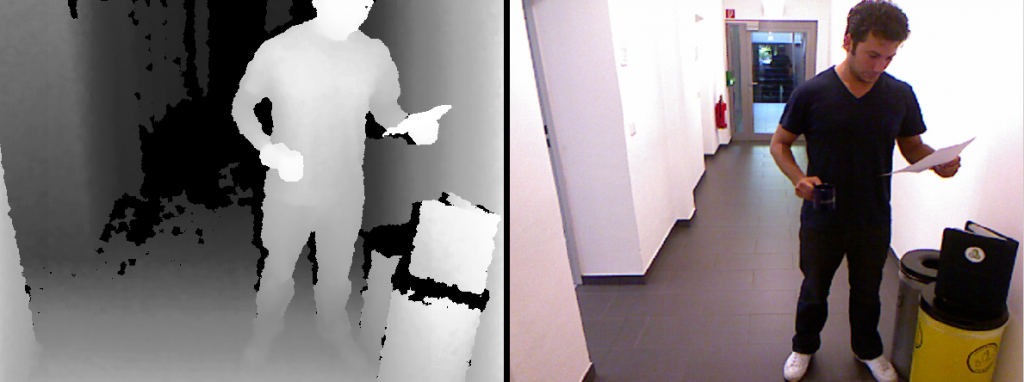
\includegraphics[width=0.9\textwidth]{kinect1_cropped-1024x382.png}
    \caption{Esimerkki Kinectin syvyyskuvasta (vasemmalla) ja värikuvasta (oikealla). \citep {kinectkuva}}
    \label{fig:kinectkuva}
  \end{center}
\end{figure}

\subsection{Eleentunnistus video- ja 3D-videokuvalta}

Eleentunnistus videokuvalta noudattaa tavallisia hahmontunnistuksen vaiheita: esikäsittely, piirrevalinta ja
luokittelu. Eleentunnistuksen erityishaasteet on huomioitava eri tavoin eri työvaiheissa. 3D-videokuva tuo 
oman lisänsä, mutta se ei merkittävästi muuta työvaiheita. Eleentunnistus on hahmontunnistuksen termein
luokitusongelma eli mahdolliset luokat tunnetaan ennalta. \citep{6239178}  \\

Esikäsittelyvaiheessa videokuvalta poistetaan häiriötä, jotka voisivat haitata eleentunnistusta.
Näitä voivat olla esimerkiksi kuvassa esiintyvät ylimääräiset objektit tai videokuvan virheet kuten kohina.
Kuvaa voidaan myös pienentää tai pakata laskennan nopeuttamiseksi. Esikäsittelyssä pyritään usein myös erottamaan ihmishahmo taustasta. Tämä on haastavaa, sillä
ihmishahmo ei välttämättä erotu esimerkiksi väritykseltään taustasta. Kinectin syvyyskameran avulla taustan irrotus onnistuu kuitenkin luotettavammin kuin pelkän 
värikuvan avulla. Ihmishahmon erottaminen taustasta helpottaa tunnistusta, sillä tällöin ihminen ei sekoitu taustaansa tai mitään taustassa olevaa
esinettä ei erehdytä pitämään ihmisen osana. Esikäsittelyssä voidaan suorittaa myös jonkinlaista ajallista jakoa videolle. Videokuvaa
voidaan esimerkiksi jakaa ajallisiin jaksoihin perustuen videokuvan samankaltaisuuteen. Ajallisen jaon 
tarkoitus on auttaa hahmottamaan kuvalla tapahtuvaa liikesarjaa ja näin helpottaa tunnistusta. \citep{6239178} \\

Hahmontunnistuksessa ratkaiseva vaihe on usein oikeiden piirteiden valinta eli piirreirrotus. Videokuvasta voidaan valita piirteeksi esimerkiksi 
tietyn suuntainen liike ajan funktiona. Liike näkyy peräkkäisten pysäytyskuvien välisenä erona. Tutkimalla liikettä
videokuvat voidaan tiivistää liikekuviin, joita voidaan luokitella yksinkertaisilla luokittelualgoritmeillä. 
Videokuvaa voidaan tarkastella myös yksittäisten pysäytyskuvien kautta. 
Tällöin voidaan hyödyntää valokuvien tunnistuksessa käytettyjä menetelmiä.
Pysäytyskuvista voidaan arvioida kontrastivaihteluita ja sitä kautta hahmottaa viivoja tai muotoja kuvassa. \citep{6239178}  \\

Tunnistusvaiheessa näytteitä verrataan opetusdatan kuvaamiin luokkiin. Tunnistusmenetelmä riippuu valituista piirteistä.
Jos videokuvaa käsitellään kokonaisuutena esimerkiksi liikekuvan avulla, kuvia voidaan luokitella yksinkertaisilla luokittelualgoritmeillä. 
Näitä voisivat olla esimerkiksi k-lähimmän naapurin luokitin. Jos videokuva esitetään yksittäisillä pysäytyskuvilla, 
on tunnistuksessa huomioitava videon aikaulottuvuus. On käytettävä rakenteellista mallia, jonka avulla voidaan tarkastella piirteen arvoa
tietyllä ajanhetkellä. Tähän tarkoitukseen on erilaisia graafisia malleja, joita esitellään tarkemmin luvussa kolme. \citep{6239178} \\

Luokittelun jälkeen menetelmälle lasketaan virheprosentti. Virheprosentti lasketaan testidatan avulla.
Testidatassa on opetusdatan tavoin tiedossa näytteiden oikeat luokat, jolloin on mahdollista laskea, kuinka suuri prosentti
näytteistä on luokiteltu oikeisiin luokkiin. Menetelmää voidaan kehittää edelleen kokeilemalla erilaisia
opetusdatajoukkoja ja valitsemalla joukko, joka tuottaa pienimmän virheprosentin testidatalle. \citep{6239178} 

\section{ChaLearn Gesture Challenge -kilpailu}
\label{ChaLearn Gesture Challenge -kilpailu}

\subsection{Kilpailun esittely}
ChaLearn Gesture Challenge -kilpailun tarkoituksena oli lisätä kiinnostusta eletunnistukseen syvyyskameralla.
Kilpailun järjesti ChaLearn-yhteisö. ChaLearn-yhteisö on useiden eri yliopistojen asiantuntijoista koostuva yhdistys,
jonka tavoitteena on herättää kiinnnostusta koneoppimiseen ja hahmontunnistukseen. \citep{kilpailunnettisivut} Kilpailu alkoi vuoden 2011 lopuilla ja se päättyi loppuvuonna 2012. Kilpailuun osallistui ensimmäisellä kierroksella 50 ryhmää,
pääasiallisesti yliopistojen tutkimusryhmiä. Kilpailijoille annettiin tietokanta, joka sisälsi 50 000 Kinect-sensorilla kuvattua videonäytettä. 
Videonäytteet sisälsivät yksittäisiä eleitä, esimerkiksi viittomia tai poliisin käsimerkkejä. Kilpailijoiden tarkoitus oli kehittää eleentunnistusmenetelmä, 
jonka avulla eleet opitaan yhdestä opetusnäytteestä. Eleitä oli jaettu kategorioihin käyttötilanteen mukaan. Esimerkiksi poliisin käsimerkit olivat yksi kategoria.
\citep{6239178} \\

Annetuilla videonäytteillä esiintyi aina yksi ihminen kerrallaan suorittamassa tiettyä elettä. Kuva rajattiin yläruumiiseen ja eleet tehtiin
pääasiallisesti käsillä. Liikkeet lopetettiin ja aloitettiin aina samasta lepoasennosta. Videonäytteet sisälsivät syvyyskamerakuvan sekä värikuvan, 
mutta eivät ranganseurausta tai muuta valmista hahmontunnistustietoa. Haasteita toivat vaihtelevat taustat ja valaistukset videokuvalla.  \citep{6239178}\\

Kilpailijoille jaettiin kolme datajoukkoa: opetusdata, validointidata ja lopullinen arviointidata. 
Opetusdatan näytteille tarjottiin oikeat luokat, joiden avulla järjestelmän opetus onnistui.
Sekä validointidatassa, että lopullisessa arviointidatassa jokaisesta eleestä annettiin ainoastaan yksi opetusnäyte eli näyte,
jolle oli paljastettu oikea luokka. Kilpailun erityishaasteena olikin yhdestä otoksesta oppiminen (One Shot Learning). 
Tarkoituksena oli kehittää järjestelmä, joka oppii tunnistamaan eleet mahdollisimman pienestä määrästä opetusdataa. 
Kilpailijoiden odotettiin soveltavan tässä siirtovaikutusoppimista (Transfer learning). \citep{6239178} \\

Siirtovaikutuksen ajatus on, että aiemmin opittuja tietoja hyödynnetään seuraavassa oppimistehtävässä. Tässä jäljitellään  
ihmisen oppimiskykyä. Ihminen oppii nopeasti tunnistamaan uusia hahmoja, jos hänellä on kokemusta vastaavista tehtävistä.
Siirtovaikutuksessa tietoja siirretään edellisestä oppimisprosessista uuteen oppimistehtävään.
Siirretyt tiedot saattavat olla esimerkiksi aiemmassa opetustehtävässä valitut piirteet tai jopa yksittäisiä datanäytteitä. \citep{5288526}\\

Järjestelmä, jonka avulla kilpailijat pystyivät testaamaan menetelmäänsä validointidataa vastaan, oli auki koko kehitysjakson ajan.
Varsinainen testidata, joilla kilpailutöitä arvosteltiin paljastettiin vasta kilpailun lopuksi. Kilpailijoilla oli muutama päivä aika
testata menetelmäänsä lopullista testidataa vastaan. Testidata sisälsi eri eleitä kuin opetusdata, mutta samoista kategorioista.
Kilpailijoiden oli siis opetettava menetelmänsä uudelleen lopullisen testidatan avulla. Kilpailijoita pyydettiin lopuksi
palauttamaan lista, joka sisälsi oikeat luokat testidatalle esitettynä merkkijonona. Lopullinen virheprosentti saatiin laskemalla Levensteinin etäisyys
oikeita luokkia kuvaavan merkkijonon ja kilpailijoiden antaman vastausmerkkijonon välillä. \citep{6239178} 


\subsection{Katsaus kilpailutöihin}
\subsubsection {Ensimmäinen kierros}
Kilpailijoiden metodeja selvitettiin ensimmäisen kierroksen jälkeen lyhyellä kyselyllä, johon vastasi 20 ryhmää 22 parhaan ryhmän joukosta.
Ryhmiltä kysyttiin muun muassa minkälaista esikäsittelyä he olivat tehneet videokuvalle, minkälaista tunnistusmenetelmää tai mitä piirteitä oli käytetty ja
mikä oli heidän menetelmänsä suoritusaika. Kyselyn tarkoituksena oli saada yleiskatsaus kilpailutöihin, sillä monet kilpailijat eivät
halunneet julkaista yksityiskohtaista kuvausta menetelmästään kilpailun ollessa vielä kesken. \citep {6239178}. \\

Vastauksista kävi ilmi, että lähes kaikki ryhmät tekivät jonkinlaista kuvan esikäsittelyä. Videokuvasta poistettiin häiriötä, asiaankuulumattomia 
kohteita tai ihmishahmon tausta. Huomioitavaa on kuitenkin, että jotkin hyvin menestyneistä ryhmistä eivät tehneet minkäänlaista esikäsittelyä kuvalle.
\citep {6239178}\\

Suurin osa osallistujista käytti HOG/HOF-piirteitä (Histogram of oriented Gradients/ Histogram of Flow), SIFT/STIP-piirteitä 
(Scale Invariant Feature Transformation/Space-time interest points), 
kulmien tai nurkkien tunnistusta tai kehitti omia, tälle datalle soveltuvia piirteitä.\citep {6239178}\\

Käytetyt piirteet perustuvat pääosin kuvan värityksen intensiteettivaihteluun.
Esimerkiksi HOG-piirteet kuvaavat kuvan intensiteettivaihtelun gradienttien suuntaa. Kuva jaetaan pieniin alueisiin, soluihin, 
joissa tarkastellaan alueen värityksen intensiteettivaihtelua. Soluille lasketaan intensiteettivaihtelun gradienttien suuntien histogrammi. 
Ajatuksena on päätellä, minkä suuntaisia viivoja tai nurkkia alueelta voidaan erottaa. \citep {1467360} Histogrammit kertovat kuvassa esiintyvistä
muodoista, eivätkä ne ole riippuvaisia hahmon sijainnista kuvassa tai kuvan yleisestä värimaailmasta.
HOG-piirteet soveltuvatkin hyvin tämänkaltaiseen hahmontunnistusongelmaan, jossa kohteen sijainti ja väritys voivat vaihdella kuvalla.
HOF-piirteet toimivat samoin kuin HOG-piirteet, paitsi yksittäisten kuvien sijaan ne tutkivat peräkkäisten kuvien vaihtelua eli liikettä videolla \citep{Pers20101369}.\\

SIFT-piirteet toimivat HOG-piirteitä hienostuneemmin valiten kuvista tärkeät pisteet. Tärkeät pisteet valitaan niin, että ne ovat riippumattomia
kuvan muutoksista kuten kiertämisestä tai skaalauksesta. Esimerkiksi kuvassa, jossa näkyy ovi, tärkeitä pisteitä voisivat olla oven kulmat.
Vaikka kuvaa kierrettäisiin tai sen kokoa muutettaisiin, tärkeät pisteet eli kulmat voidaan löytää kuvasta.
Pisteiden valinnassa hyödynnetään värityksen intensiteettivaihtelua ja tilastollisia menetelmiä.  \citep {790410}
STIP-piirteet perustuvat samankaltaiseen menetelmään, mutta huomioivat myös videon aikaulottuvuuden \citep{1238378}. \\

Piirteitä voidaan tutkia syvyys- ja värikuvasta. Syvyyskuvan etu verrattuna värikuvaan on, että siinä
ei esiinny värejä tai tekstuureja, jotka häiritsisivät hahmon erottumista tai videoiden vertailua.
Suurin osa kilpailijoista käyttikin töissään pelkkää syvyyskuvaa. Osa käytti sekä väri- että syvyyskuvaa. 
Mielenkiintoista on, että ensimmäisen kierroksen toisen sijan voittaja käytti työssään pelkkää värikuvaa. 
Kaikki kilpailijat käyttivät jonkinlaista piirteiden tiivistystä tai kuvausta toiseen lineaariavaruuteen. \citep {6239178}\\ 

Ajallisen rakenteen mallintamiseen käytettiin erilaisia graafisia malleja kuten Markovin piilomuuttujaa ja Conditional Random Fields -menetelmää.
Kaikki tunnistustusmenetelmät eivät kuitenkaan huomioineet videon ajallista rakennetta. \citep {6239178}\\ 

Markovin muuttuja kuvaa havainnon sarjana tiloja eli tässä tapauksessa videon sarjana pysäytyskuvia. 
Tilat esitetään sopivien piirteiden avulla eli esimerkiksi kuvat voidaan esittää HOG/HOF-piirteiden avulla. 
Menetelmä kertoo kuinka todennäköisesti annettu havainto kuuluu tiettyyn luokkaan. 
Ajatuksena on, että annetun havainnon luokka on tuntematon, mutta se voidaan löytää sen etsimällä todennäköisin luokka. 
Luokat saadaan opetusdatasta.\\

Luokkien tiheysfunktiot lasketaan suurimman todennäköisyyden
(Most Likelihood) -menetelmällä. Kyseessä on Bayesilainen menetelmä eli jakauma tunnetaan, mutta ei parametreja.
Parametrien arvot optimoidaan niin, että todennäköisyys opetusliikkeelle kuulua kuvaamaansa luokkaan on mahdollisimman suuri.
Luokan tiheysfunktion avulla voidaan laskea kuinka todennäköisesti tietty tilasarja esiintyy tässä luokassa.
Luokassa on kuitenkin useita mahdollisia tilasarjoja. Todennäköisyys annetulle havainnolle $O = O_{1}, O_{2}...O_{n}$ kuulua 
luokkaan $\lambda$ saadaan siis seuraavasti:
\begin{equation}
P(O,Q|\lambda) = \sum\limits_{kaikki Q:t}P(O|Q, \lambda)P(Q|\lambda)
\end{equation}
jossa $Q = Q_{1}, Q_{2} ... Q_{n}$ eli Q on määrätyn mittainen tilasarja. Todennäköisyys havainnolle O esittää
tiettyä tilasarjaa Q kerrotaan todennäköisyydellä $P(Q|\lambda)$ eli todennäköisyydellä tilasarjalle Q esiintyyä luokassa $\lambda$. 
Lopuksi summataan yhteen todennäköisyydet sarjalle O kuulua luokkaan $\lambda$ kaikilla tilasarjoilla Q. 
Näin saadaan lopullinen todennäköisyys havainnolle O kuulua luokkaan $\lambda$. On huomioitava, että menetelmä vaatii
kaikkien näytteiden olevan samanpituisia eli koostuvan tietystä ennalta määrätystä määrästä tiloja. Tämä saattaa asettaa
rajoituksia menetelmän sovelluksissa.\citep {18626}\\

Conditional Random Fields -menetelmä perustuu samankaltaiseen intuitioon. Lähtökohta molemmissa on, että yksittäisen 
datapisteen sijaan luokitellaan datajoukkoja, joilla on sisäinen, tässä ajallinen, rakenne. \citep {1315232}\\

Kilpailutöissä, joissa ei käytetty edellämainittuja ajallisen rakenteen mallintamista menetelmiä, 
luokittelussa käytettiin k-lähimmän naapurin luokitinta tai muita yksinkertaisia luokittelumenetelmiä. \\

Kilpailun järjestäjien odottamaa metodia, siirtovaikutusta käytettiin vähäisesti, eikä kukaan menestyneistä kilpailijoista käyttänyt sitä.
Kilpailun varsinainen haaste, yhdestä eleestä oppiminen, jäi siis vähemmälle huomiolle. \citep {6239178} \\

Kahdeksan menestyneintä työtä esitellään taulukossa ~\ref{table:dvbt_param}. Taulukosta huomataan, että parhaiten menestyneiden töiden
joukossa suurin osa käytti tunnistuksesa menetelmää, joka huomioi videon ajallisen rakenteen. Tällöin videokuvasta valitaan piirteet, joiden
muutosta seurataan ajan funktiona. Poikkeuksen tekevät ryhmät Zonga ja Xiaozhuwudi, joiden menetelmä perustuu videon käsittelyyn erilaisten liikekuvien avulla. 
\citep {6239178}\\

\begin{table}[th]
\caption{ChaLearn Gesture Challenge -kilpailun kahdeksan parhaiten sijoittunutta ryhmää}
\label{table:dvbt_param}
\begin{center}
\begin{tabular}{|p{0.35\textwidth}|p{0.45\textwidth}|} 
    \hline
Ryhmän nimi & Menetelmä \\
    \hline
    \hline
Alfnie & Motion Signature analyses\\ 
    \hline
Pennect & Markovin piilomallin tapainen menetelmä ja HOG/HOF-piirteet.\\
    \hline
One Million Monkeys & Markovin piilomalli ja kulmien tunnistus\\
    \hline
Immortals & Markovin piilomalli ja HOG/HOF-piirteet\\
    \hline
Zonga & Pienimmänneliösumman menetelmä ja HOSVD -menetelmä\\
    \hline
Balazs Godeny & Thumbnail Dynamic Time Warping” (DTW) ja HOG/HOF-piirteet sekä kulmien tunnistus.\\
    \hline
SkyNet & Dynamic Time Warping(DTW) ja kulmien tunnistus\\
    \hline
Xiaozhuwudi & MHI-kuva johon on lisätty GEI- ja INV-kuvat\\
    \hline	
\end{tabular}
\end{center}
\end{table}

\newpage
\subsubsection {Toinen kierros}

Kilpailun toinen kierros toteutettiin samoilla järjestelyillä kuin ensimmäinen. Koska kierros loppui
vasta tämän kandinaatintyön kirjoittamisen aikoihin, on se jätetty työssä vähemmälle tarkastelulle.\\

Toisen kierroksen jälkeen kilpailijoiden metodeja selvitettiin kyselyllä samoin kuin ensimmäisen
kierroksen jälkeen. Kyselyyn vastasi 28 ryhmää. Vastausten perusteella toisella kierroksella menestyneet 
menetelmät olivat hyvin samantapaisia kuin ensimmäisen kierroksen menestyneet menetelmät. HOG/HOG-piirteet sekä muut
kuvan intensiteettivaihteluihin perustuvat piirteet yhdistettynä Markovin piilomuuttujaan tai muuhun
vastaavaan malliin olivat suosituin menetelmä. \citep{chalearn2}\\

Molemmilla kierroksilla oli sama voittaja, ryhmä Alfnie. 
Voittajaryhmä väittää työnsä matkivan ihmisen hahmontunnistuskykyä. Työtä ei ole kuitenkaan vielä tämän kandinaatintyön kirjoittamisen aikaan julkaistu,
 joten siihen ei päästä tutustumaan tarkemmin. Työ perustuu
ryhmän ilmoituksen mukaan jonkinlaiseen mukautettuun Markovin piilomuuttujaan. Mielenkiintoista on,
että huolimatta hyvästä luokittelukyvystään menetelmä oli myös yksi kilpailun nopeimmista. Vaikka menetelmä oli siis 
luokittelumielesssä tehokas, se ei kuitenkaan ollut laskennallisesti erityisen raskas. \citep{chalearn2}\\

Toisen kierroksen toiseksi sijoittunut, ryhmä Turtle Tamers, käytti samankaltaista menetelmää kuin 
ensimmäisen kierroksen toisen sijan voittaja, ryhmä Pennect. Molemmat ryhmät käyttivät HOG/HOF-piirteitä sekä Markovin piilomuuttujaa. 
Kolmannen sijan saavuttanut ryhmä Joewan sen sijaan käytti hyvin erilaista menetelmää. Ryhmä käytti Bag of MOSIFT -piirteitä 
yhdistettynä lähimmän naapurin luokittimeen. \citep{chalearn2} Bag of MOSIFT -piirteet on muokattu versio
yleisestä Bag of features -menetelmästä. Bag of features -menetelmät kuvaavat tietyn piirteen avulla
kuinka usein jokainen arvo esiintyy näytteessä. Ne mittaavat siis ainoastaan kuinka usein tietty arvo esiintyy näytteessä eivätkä 
välitä näytteen sisäisestä rakenteesta. \citep{bagoffeatures} \\

Varsinaisen validoinnin lisäksi kilpailutöille suoritettiin palautuksen jälkeen vielä yksi testaus. Tässä testauksessa tutkittiin kuinka 
hyvin kilpailijoiden menetelmät tunnistivat eleen, jos videokuvaa oli tietoisesti käännetty hieman. Oikeissa sovelluksissa on tärkeää,
että ele pystytään tunnistamaan, vaikka se eroaisi hieman alkuperäisestä näytteestä esimerkiksi kuvakulmaltaan. 
Tässäkin testissä voittajaryhmä menestyi hyvin, kun taas esimerkiksi kaksi seuraavaa ryhmää menestyivät manipuloidulla datalla huomattavasti
huonommin kuin varsinaisella kilpailudatalla. Tämä lisää ennestään mielenkiintoa voittajatyötä kohtaan. \citep{chalearn2}


\section {Katsaus eräisiin menestyneisiin kilpailutöihin}

Tässä luvussa esitellään kolme menestyneistä töistä tarkemmin. Työt ovat eräitä esimerkkejä toimivista ratkaisuista. Ne on valittu tähän, 
koska ne edustavat erilaisia näkökulmia ongelmaan. Valintamahdollisuuksia rajoitti se, että kaikki kilpailijat eivät olleet vielä julkaisseet 
menetelmäänsä tämä työn kirjoittamisen aikana. Kolmesta valitusta työstä yksi, Immortals edustaa kilpailun yleislinjaa ja kaksi muuta valittua työtä,
Zonga ja Xiaozhuwudi ovat esimerkkeinä omaperäisemmistä menetelmistä.\\

\subsection{Ryhmä Xiaozhuwudi ja laajennettu MHI-menetelmä}
Ryhmä Xiaozhuwudi lähti liikkeelle MHI eli Motion History Image -menetelmästä \citep {6239179}. MHI-kuva esitää liikkeen määrän videokuvalla.
Videopätkä tiivistetään yhteen liikekuvaan, joka kuvaa liikkeen viimeaikaisuutta. Kohdat, joissa videokuvalla on ollut
liikettä esitetään harmaasävyillä. Mitä viimeaikaisempaa liike on ollut sitä valkoisempana se näkyy kuvassa. Liikkumattomat
alueet näkyvät täysin mustana. Videokuvalta tutkitaan siis vain liikettä, eikä pyritä esimerkiksi tunnistamaan kuvalla olevia kohteita
tai ihmiskehon osia. Tämä menetelmä matkii ihmisen tapaa tunnistaa eleitä. Ihminen tunnistaa erittäin hyvin inhimilliset eleet  
sumealtakin videokuvalta vaikka ei yksittäisestä pysäytyskuvasta tunnistaisi edes ihmishahmoa. \citep {910878}  \\

\begin{figure}[htb]
  \begin{center}
    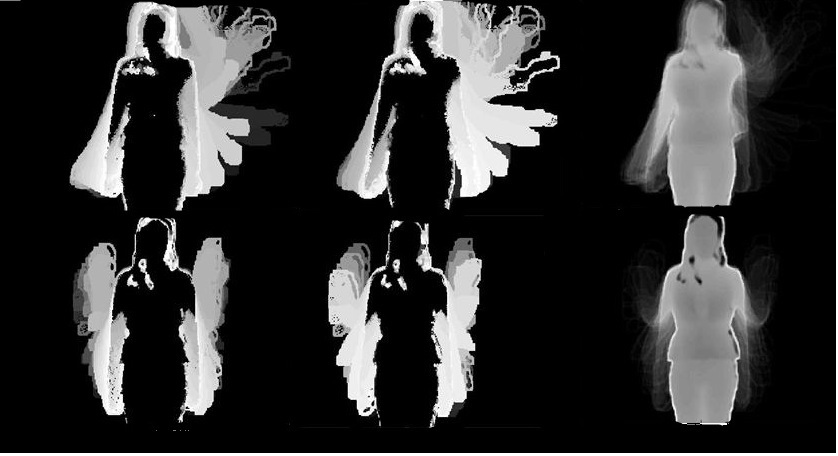
\includegraphics[width=0.9\textwidth]{mhi_ex.jpg}
    \caption{Kuvassa vasemmalta oikealle MHI-, INV- ja MEI-kuva. \citep {6239179}}
    \label{fig:mhiinvmei}
  \end{center}
\end{figure}

Xiaozhuwudi-ryhmä tunnistaa MHI-kuvassa kuitenkin ongelmia. MHI-kuvan avulla on vaikeaa tunnistaa eleitä, jotka sisältävät toistuvaa liikkeitä, 
esimerkiksi vilkutusta.
Liikkeen toistuessa MHI-kuva muuttuu helposti sekavaksi ja on vaikea erottaa tarkkaa liikerataa. Ryhmä ehdottaakin MHI-kuvan laajentamista 
INV(Inversed Recording)- ja GEI(Gait Energy Image)-kuvilla. INV-kuva on MHI-kuvalle käänteinen kuva. INV-kuvassa katsotaan videokuvaa alusta loppuun päin.
Mitä aikaisemmin liike esiintyy videolla sitä vaaleampana se näytetään kuvassa. INV-kuvan avulla saadaan kuvaus videon alkutilanteesta, mikä täydentää MHI-kuvaa. 
GEI-kuva esittää paikallaan pysyviä kohteita. Mitä enemmän kohde on paikoillaan videolla sitä vaaleampana tämä alue näkyy kuvassa.
Kohdissa joissa on liikettä, näkyy harmaa sävyä ja täysin paikallaan olevat kohteet ovat valkoisia. Tausta on erotettu kohteesta ja jätetty mustaksi. 
GEI-kuvan avulla liikkeestä saadaan hyvä kokonaiskuva ja se on hyödyllinen etenkin toistuvan liikkeen tunnistuksessa. \citep {6239179} \\

Kuvassa ~\ref{fig:mhiinvmei} on esitetty kahdelle
liikkeelle MHI-, INV- ja GEI-kuvat. Kuvat havainnollistavat hyvin miten INV- ja GEI-kuvat
täydentävät MHI-kuvaa. Pelkän MHI-kuvan perusteella on vaikea erottaa liikkeet toisistaan.
INV- ja GEI-kuvien avulla liikkeet erottuvat kuitenkin selkeämmin. \\

Datan esikäsittelyssä Xiaozhuwudi hyödynsi Kinectin syvyyskuvaa poistamalla taustan ihmishahmolta. Lisäksi esikäsittelyssä poistettiin häiriöitä.
MHI-, GEI- ja INV-kuville suoritettiin dimensioiden vähennys ja piirreirroitus. Eleiden tunnistukseen käytettiin Maximum Correlation Coeffient -luokittelijaa,
joka perustuu kuvien väliseen korrelaatioon. \citep{6239179}\\

Ryhmä väittää työnsä suoriutuvan eleentunnistusongelmasta huomattavasti nopeammin kuin muut paikalliseen tietoon perustuvat eleentunnistusmenetelmät \citep{firstround}.
Lisäksi ryhmän esittämä luokittelualgoritmi vastaa ryhmän mukaan paremmin yhdestä eleestä oppimisen -haasteeseen kuin esimerkiksi Markovin piilomuuttujaan perustuvat menetelmät
\citep{6239179}.

\subsection{Ryhmä Immortals ja Markovin piilomuuttuja}

Ryhmä Immortals esittää kilpailutyössään oletuksen, että ele koostuu ennen kaikkia useista yksittäisistä liikkeistä. 
Sen mukaan eleet tunnistetaan parhaiten käsittelemällä elettä sarjana liikkeitä. Tämä eroaa ryhmän mukaan tyypillisestä 
tavasta lähestyä ongelmaa. \citep {6239185}\\

Ryhmä lähti liikkeelle opetusvaiheessa yksittäisistä liikkeistä. Yksittäisille liikkeille luodaan allekirjoitus eli malli,
jonka avulla ne voidaan tunnistaa. Allekirjoituksen luominen on monivaiheinen operaatio. Ensin kuvista poimitaan niin sanotut
tärkeät pisteet eli pisteet joilla on merkitystä liikkeen tunnistamisen kannalta. Tässä Immortals hyödynsi Kinectin syvyyskuvaa.
Immortals arvioi, että ne kohdat kuvasta, joissa on tapahtunut syvyyssuuntaista muutosta syvyyskameran kuvassa ovat kyseisen videon pysäytyskuvan
tärkeitä pisteitä. Tärkeille pisteille lasketaan HOG(Histogram of Oriented Gradients)- ja HOF(Histogram of Flow)-histogrammit. 
Tämän jälkeen kaikkien kuvien kaikki histogrammit ryhmitellään tavallisen ryhmittelyalgoritmin avulla.
Histogrammeja kutsutaan ryhmittelyn jälkeen "visuaalisiksi sanoiksi". Yhdessä ryhmässä ovat kaikki tietyn sanan esiintymät.
Tarkoituksena on tutkia visuaalisten sanojen esiintymistä yhdessä ja muodostaa niistä aihepiirejä. 
Yksittäistä pysäytyskuvaa voidaan kuvata sillä, mitä sanoja ja mistä aihepiireistä siinä esiintyy. \citep {6239185}\\

Liikkeelle luodaan sanojen perusteella perusteella malli, jota käytetään tunnistusvaiheessa. Mallin perustana on Markovin piilomuuttuja
eli HMM (Hidden Markov Model). Koska tutkitaan kahta piirrettä, HOG- ja HOF-piirrettä, käytetään monikanavaista Markovin piilomuuttujaa eli McHMM (Multi Channel Hidden Markov Model). 
HOG- ja HOF-piirteet paljastavat erilaista tietoa havainnosta ja tukevat tässä hyvin toisiaan. McHMM-muuttujan parametreja ovat alkutila, 
todennäköisyys tilojen väliselle siirtymälle sekä tilan todennäköisyys ja tilan kuvaus visuaalisten sanojen eli HOG- ja HOF-piirteiden avulla. 
Tilalla tarkoitetaan tässä yksittäistä pysäytyskuvaa. Malli opetetaan parametrien avulla niin, että se tunnistaa tietyn liikkeen eli tietyn
sarjan pysäytyskuvia.\citep {6239185} Kuvassa ~\ref{fig:HMM} on tarkennettu vielä Markovin piilomuuttujan toimintaa. Kuvassa on 
esitetty havainto ja Markovin piilomuuttujan mahdolliset tilat, sekä niiden väliset siirtymätodennäköisyydet. Tarkoitus on löytää
tilasarja, joka todennäköisimmin on muodostanut tämän havainnon. Parametrit eli tilat ja todennäköisyydet on opetettu mallien perusteella. \\

\begin{figure}[htb]
  \begin{center}
    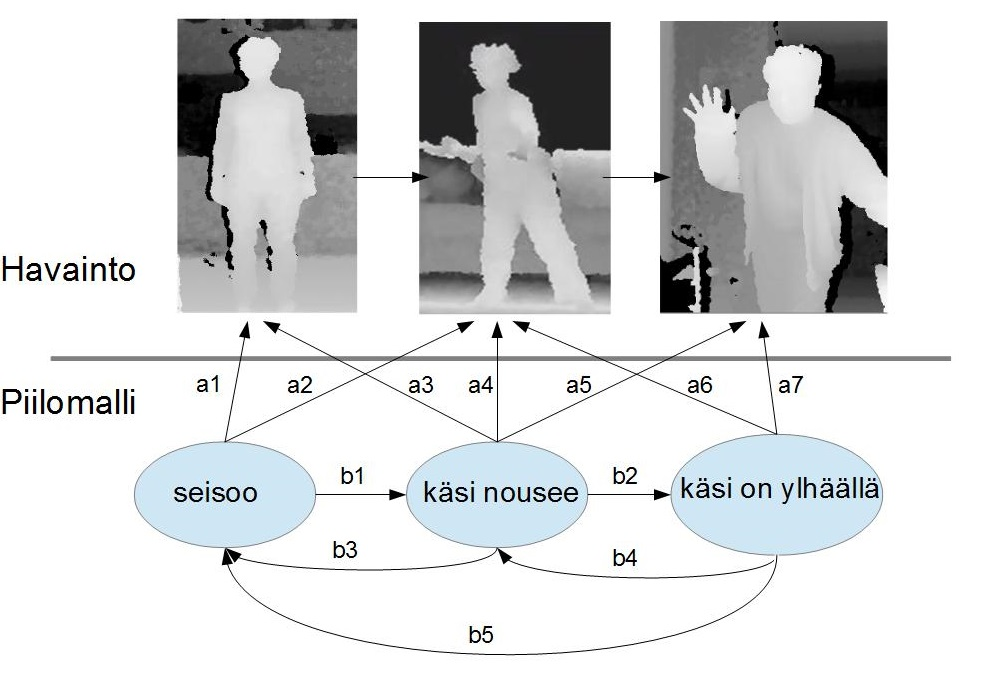
\includegraphics[width=0.9\textwidth]{HMModfcropped.jpg}
    \caption{Markovin piilomuuttujan käyttö eleentunnistuksessa. Viivan yläpuolella havainto on esitetty pysäytyskuvien avulla. Viivan alapuolella
	ovat mahdolliset tilat,	sekä niiden väliset siirtymätodennäköisyydet b1-bn. Todennäköisyydet a1-an kuvaavat kuinka todennäköisesti tila esittää havaittua tilaa.
	Tarkoituksena on löytää tilasarja, joka kaikkein todennäköisimmin muodostaa havainnon. Kuvan esittämässä tilanteessa todennäköisin tilasarja
	olisi varmaankin: seisoo, käsi nousee, käsi on ylhäällä. On huomioitava, että oikessa tilanteessa tutkitaan täysin perättäisiä pysäytyskuvia, kun
	tässä esitetyt kuvat ovat selkeyden vuoksi liikkeen eri vaiheista.}
    \label{fig:HMM}
  \end{center}
\end{figure}

Tunnistusongelma pelkistyy lopulta kysymykseen: Mikä liikesarja kaikken todennäköisimmin on muodostanut tämän videonäytteen?
Tämän tyylinen ongelma voidaan ratkaista Viterbin algoritmillä. Tämä vaatii kuitenkin, että ele rajataan koostumaan tietystä määrästä liikkeitä.
Tässä tapauksessa on määritelty, että jokainen elenäyte sisältää viisi liikettä.
Viterbin algoritmi pyrkii löytämään todennököismmän polun eri liikkeiden välillä. Algoritmi käy videota läpi liike kerrallaan ja laskee mikä
on mallien perusteella todennäköisin liike. Lopuksi saadaan liikesarja, josta videonäyte todennäköisimmän koostuu.
Liikesarja liitetään tunnistusvaiheessa tiettyyn eleeseen. On huomiotava, että Viterbin algoritmiä käytetään ryhmän menetelmässä 
kahdella tasolla. Menetelmän alimmalla tasolla algoritmiä käytetään Markovin piilomuuttujan kanssa tunnistamaan yksittäinen liike pysäytyskuvien perusteella. 
Toisaalta Viterbin algoritmiä käytetään myös ylemmällä tasolla tunnistamaan todennäköisin liikesarja eli ele liikkeiden perusteella. \citep {6239185}\\

Ryhmä Immortals kertoo lähestymistapansa olevan peräisin puheentunnistusmenetelmistä. Ryhmä on kokeillut menetelmää menestyksekkäästi myös muille videotietokannoilla,
jotka sisälsivät pelkää värivideokuvaa. \citep{firstround}\\


\subsection{Ryhmä Zonga ja pienimmän neliösumman menetelmä sovelluttuna monistoon}
Ryhmä Zonga käyttää kehittämäänsä menetelmää, joka soveltuu yleisesti videokuvan luokitteluun. 
Menetelmää on hieman mukautettu eleentunnistusta varten, mutta lähtökohdiltaan se on hyvin 
matemaattinen eikä juuri hyödynnä perinteisiä kuvankäsittelymenetelmiä. \citep {6239180}\\

Videokuva on helppo mieltää kolmiulotteiseksi datajoukoksi. Videokuvan ulottuvuuksia ovat korkeus, leveys ja aika.
Ryhmä Zonga käsitteleekin videokuvaa kolmiulotteisena tensorina. Tensorin ulottuvuudet vastaavat videon ulottuvuuksia.
Voidaan ajatella, että yksi matriisi kuvaa yhtä pysäytyskuvaa, jolloin tensorin tuoma kolmas ulottuvuus on aikaulottuvuus. \citep {6239180}\\

Tensorin käsittely sellaisenaan on hankalaa sen suuren datamäärän vuoksi. Helpottaakseen videon käsittelyä
ryhmä laskee tensorille HOSVD(Higher-order singular value decomposition)-hajotelman. Hajotelma on muokattu versio
singulaarihajotelmasta. Hajotelma avaa tensorin kolmeksi matriisiksi.
Matriisit kuvaavat videon vaakasuoraa liikettä, pystysuoraista liikettä ja summakuvan videon yli. \citep {HOSVD} 
Tensori hajotetaan tekijöihinsä aputensorin (Core Tensor) S avulla:

\begin{equation}
A = S *_{1} V_{appearance}^{(1)} *_{2} V_{h-motion}^{(2)} *_{3} V_{v-motion}*^{(3)}
\end{equation}

jossa A on havaintomatriisi, S on aputensori ja V-matriisit ovat tensorin hajotelma. $V_{appereance}$-matriisi on
videon summakuva ajan yli. $V_{h-motion}$-matriisi kuvaa vaakasuuntaista liikettä videolla ja $V_{v-motion}$-matriisi
kuvaa pystysuoraa liikettä videolla. Kuvassa ~\ref{fig:hosvdhajotelma} esitetty hajotelman matriisit pikselikuvina.
Kuvasta nähdään selkeästi, että matriisihajotelman tekijät esittävät liikkeen kolmena kuvana. \citep {6239180}\\

\begin{figure}[htb]
  \begin{center}
    \includegraphics[width=0.9\textwidth]{hosvdhajotelma.png}
    \caption{Videon tensoriesitys on hajotettu HOSVD-hajotelman avulla kolmeen tekijään. Vasemmalta oikealle: summakuva koko videolle, videon vaakasuuntainen liike ja videon pystysuuntainen liike. \citep {6239180}}
    \label{fig:hosvdhajotelma}
  \end{center}
\end{figure}

Matriisihajotelman avulla video voidaan kuvata pisteenä kolmiulotteisessa monistossa (manifold). Moniston ulottuvuudet
vastaavat tensorihajotelman ulottuvuuksia. Monisto säilyttää videon 
alkuperäisen geometrisen rakenteen Euklidista avaruutta paremmin. \citep {Lui2012380} Monistokuvauksen avulla videoita voidaan käsitellä yksittäisinä
pisteinä, jolloin niiden luokittelu helpottuu. Monistojen käyttö videonkuvan kanssa ei ole uusi asia eleentunnistuksessa. 
Ryhmä Zonga kuitenkin yhdistää monistokuvaukseen pienimmän neliösumman menetelmän, joka tekee ryhmän mukaan heidän lähestymistavastaan
ainutlaatuisen.\citep {6239180}\\

Pienimmän neliösumman menetelmä on regressio-ongelma, eli siinä etsitään jonkinlaista suhdetta havainnon ja luokan välille. 
Opetusvaiheessa tunnetaan havainto ja sen luokka, joiden välille pyritään löytämään funktio. Funktiota kutsutaan regressiofunktioksi.
Tunnistusvaiheessa havaintojen luokat lasketaan regressiofunktion avaulla.\citep{leastsquares}\\

Regressio-ongelma on muotoa $y = A * \beta$, jossa $y$-vektori esittää pisteet tulosavaruudessa, A-matriisi on havaintomatriisi 
ja $\beta$-vektori on painovektori, joka kuvaa havaintomatriisin pisteet tulospisteiksi.
Opetusvaiheessa pyritään löytämään painovektori, joka kuvaa havainnon mahdollisimman lähelle oikeaa luokkaa
tulosavaruudessa. \citep {6239180} Pienimmän neliösumman menetelmässä pyritään minimoimaan luokitteluvirheen neliötä eli oikean tuloksen 
ja arvioidun tuloksen erotuksen neliötä \citep{leastsquares}.
Minimoidaan siis funktiota:
\begin{equation}
R(\beta) = ||y-A\beta||^2 \\
\end{equation}

Painovektorin avulla muodostetaan regressiofunktio, jonka avulla havainnot kuvataan samaan tulosavaruuteen kuin opetuspisteet. Havainnot
luokitellaan tämän jälkeen etäisyyden perusteella. Luokittelufunktio on muotoa:
\begin{equation}
j*=argmin_{j}D(Y,\psi_{j}(Y))
\end{equation}

jossa Y on annettu havainto, j on luokka ja $\psi_{j}$ on luokan j regressiofunktio. D-funktio laskee annetun havainnon ja regression välisen erotuksen.
Tarkoitus on löytää luokka, joka antaa pienimmän etäisyyden.\\ 

Ryhmä Zonga kertoo menetelmänsä olevan yksinkertainen ja helppo toteuttaa. 
Verrattuna muihin töihin se huomioi eyhmän mukaan erityisen hyvin eleen luonnollisen tila-avaruuden. \citep{firstround} 

\subsection{Yhteenveto ryhmien kilpailutöistä}

Ryhmä Xiaozhuwudi sijoittui kilpailussa kahdeksanneksi, ryhmä Immortals viidenneksi ja ryhmä Zonga kuudenneksi ensimmäisellä kierroksella
viidenkymmenen kilpailijan joukosta. Vaikka valitut kilpailutyöt hyödynsivät varsin erilaisia menetelmiä ja panostivat eri vaiheisiin eleentunnistuksessa,
niiden tuloksissa ei ollut huomattavaa eroa \citep{6239178}. Ryhmä Immortals edusti menetelmällään kilpailun yleistä suuntausta,
kun taas ryhmät Zonga ja Xiaozhuwudi poikkesivat kilpailun valtavirrasta. Vaikka ryhmien Zonga ja Xiaozhuwudi menetelmät olivat keskenään
kokonaisuudessaan melko erilaiset, ne muistuttivat kuitenkin toisiaan lähestymistavaltaan ja piirrevalinnan osalta.\\

Ryhmä Immortals kiinnitti menetelmässään erityistä huomioita piirreirroitukseen. Ryhmän esittämä piirreirroitus on monivaiheinen operaatio,
jossa hyödynnettiin paitsi paikkatietoa HOG-piirteiden avulla, myös liiketietoa HOF-piirteiden avulla.
Ajallisen rakenteen mallintamiseen ryhmä käyttää Markovin piilomuuttujaa. Kaksi muuta ryhmää,
Zonga ja Xiaozhuwudi mallinsivat eleitä yksittäisten summakuvien avulla ohittaen videon ajallisen rakenteen.
Molemmat ryhmät hyödynsivät tunnistuksessa ensisijaisesti liiketietoa. Summakuvat esittivät videolla tapahtunutta liikettä.
Ryhmä Xiaozhuwudi ilmoittaa tehneensä summakuville vielä HOG-piirreirroituksen ja dimensioiden vähennyksen LDA-menetelmällä (Linear Diskriminant Analysis) \citep{6239179}.
Ryhmä Zonga ei ilmoittanut muuta piirreirroitusta kuin HOSVD-hajotelman. Ryhmän Zonga menetelmä poikkeaakin piirreirroituksen osalta
muista kilpailutöistä ja tyypillisestä lähestymistavasta kuvan- tai videokuvankäsittelyssä. Tämä näkyy myös videon esikäsittelyssä. 
Ryhmät Immortals ja Xiaozhuwudi esikäsittelivät videokuvaa eli muun muuassa irrottivat ihmishahmon taustastaan videokuvalla,
mutta ryhmä Xiaozhuwudi ei tehnyt videokuvalle minkäänlaista esikäsittelyä \citep{firstround}.\\

Ryhmien käyttämät tunnistusmenetelmät heijastelivat piirrevalintoja. Ryhmät Xiaozhuwudi ja Zonga, jotka tiivistivät näytteet 
yksittäisiin kuviin käyttivät luokittelumenetelmiä, jotka perustuvat etäisyyden laskemiseen 
Euklidissa tai sen kaltaisessa tilassa. Ryhmä Immortals, joka lähti oletuksesta, että videokuva koostuu ennen kaikkea joukosta perättäisiä 
yksittäisiä liikkeitä käytti tunnistuksessa Markovin piilomuuttujaa ja Viterbin algoritmiä kahdella tasolla. Ryhmä Immortals jakoi videokuvaa 
ajallisesti Viterbin algoritmin käyttöä varten. Myös ryhmät Xiaozhuwudi ja Zonga ilmoittivat tehneensä videolle 
jonkinlaista ajallista jakoa luokittelua varten \citep{firstround}. \\

Esitellyistä töistä ryhmän Immortals työ vaikuttaa laskennallisesti raskammailta, mutta ryhmän ilmoituksen perustella laskenta-aika on vain lineaarinen suhteessa 
näytteiden määrään. Ryhmä Xiaozhuwudi ilmoitti saman lukeman. Ryhmä Zonga ilmoittaa laskenta-ajan olevan paitsi lineaarinen suhteessa näytteiden määrään myös
neliöllinen suhteessa kuvan kokoon. \citep{firstround} Tästä näkökulmasta ryhmän Zonga työ on suorituksista heikoin, sillä monet eleentunnistussovellukset vaativat 
nopeaa, lähes reaaliaikaista suoritusta. \\

Ryhmät Xiaozhuwudi ja Zonga ilmoittivat käyttäneensä työssään kilpailussa toivottua siirtovaikutusoppimista. Molemmat ryhmät ilmoittivat,
että opetusdataa oli käytetty eleiden mallintamiseen. Ryhmät eivät kuitenkaan tarkemmin esitelleet tätä näkökulmaa menetelmiensä kuvauksissa.
Ryhmä Immortals ei ilmoittanut käyttänäänsä siirtovaikutusta. \citep{firstround}\\

Kaikki kolme ryhmää hyödynsivät tunnistuksessa sekä väri- että syvyyskuvaa. Kaikki kolme kuvattua menetelmää olivat kuitenkin sellasia, 
että ne soveltuisivat ainakin pienin muokkauksin myös pelkän värikuvan luokitteluun. Mikään menetelmistä ei perustunutt ihmishahmon 
tai sen osien tunnistukseen, vaan videokuvaa käsiteltiin pikselidatana, vailla informaatiota sen esittämästä kohteesta.
Kaikki menetelmät sopisivat siis  pienin muokkauksin myös muihin videokuvan luokitteluongelmiin kuin eleentunnistukseen. Ryhmien Xiaozhuwudi ja Zonga 
menetelmät perustuivat kuitenkin lähes yksinomaan liikkeen määrään videokuvalla, joten ne eivät välttämättä soveltuisi 
kaikkiin luokitteluongelmiin.\\

Taulukossa ~\ref{table:kolmetyötä} on vielä esitetty tiivistetysti ryhmien Xiaozhuwudi, Immortals ja Zonga menetelmät.
Taulukosta näkee, miltä osin menetelmät ovat samankaltaisia ja miltä osin ne eroavat toisistaan. Siinä missä ryhmät
Zonga ja Xiaozhuwudi käyttivät piirrevalinnassa samaa lähtökohtaa (summakuvat ja liike), muistuttivat Immortals ja Xiaozhuwudi
toisiaan enemmän piirreirroituksen (HOG/HOF-piirteet) ja kuvien käsittelyn osalta. \\

\begin{table}[th]
\caption{Vertailussa ryhmien Xiaozhuwudi, Immortals ja Zonga kilpailutyöt. \citep{firstround}}
\label{table:kolmetyötä}
\begin{center}
\begin{tabular}{|p{0.15\textwidth}|p{0.25\textwidth}|p{0.25\textwidth}|p{0.25\textwidth}|} 
    \hline
 & Xiaozhuwudi & Immortals & Zonga\\
    \hline
    \hline
 Kuvan esikäsittely & Taustan poisto, melun poisto, värimaailman tasoittaminen& Taustan poisto & Ei esikäsittelyä\\
    \hline
 Piirreirroitus & HOG/HOF-piirteet & HOG/HOF-piirteet & HOSVD-hajotelma \\
    \hline
 Dimensioiden pienennys & Tekijöihin jako (LDA)& Datan ryhmittely & Tekijöihin jako (HOSV-menetelmällä)\\
    \hline	
 Ajallinen jako &Perustuu kuvan eroon lepotilan välillä &Viterbin jako &Perustuu kuvan eroon lepotilan välillä\\
     \hline
 Eleen esitys &Summakuva &Joukko piirteitä &Kolmiuloitteinen tensori (josta hajotelma liikekuviin)\\
     \hline
 Luokittelu &Maksimikorrelaatioon perustuva luokittelija &Markovin piilomuuttuja &Lähimmän naapurin luokittelija\\
      \hline
 Siirto-oppiminen &Kehitysdataa käytetty eleiden mallintamiseen&Ei huomioitu&Kehitysdataa käytetty eleiden mallintamiseen\\
      \hline
 Suoritusaika &Lineaarinen näytteiden määrään&Lineaarinen näytteiden määrään &Neliöllinen kuvan kokooon, lineaarinen näytteiden määrään\\
      \hline
	  \hline
\end{tabular}
\end{center}
\end{table}
\newpage
\section {Johtopäätökset}

Kinect-kameran ja muiden vastaavien kameroiden 3D-videokuva on tuonut ratkaisuja eleentunnistuksen ongelmiin. Yksivärinen syvyyskuva pienentää erilaisista tekstuureista
ja väreistä johtuvaa vaihtelua, jolloin luokkien sisäinen vaihtelu pienenee ja luokittelutehtävä helpottuu. Syvyyskuvan avulla
saadaa lisätietoa eleestä, jolloin toisiaan muistuttavat eleet voidaan erottaa entistä varmemmin. Syvyyskamera on jo itsessään
helpottanut eleentunnistusta ja saattaa antaa parempia tuloksia vanhoilla, jo tunnetuilla eleentunnistusmenetelmillä. Uusia menetelmiä
pyritään kuitenkin kehittämään, jotta syvyyskameran saadut edut saataisiin entisestä paremmin hyödynnettyä.\\

ChaLearn Gesture Challenge -kilpailun kilpailutöiden perusteella 3D-videokuvan tunnistuksessa käytetäänkin pitkälti samoja 
menetelmiä kuin 2D-videokuvan tunnistuksessa. Kilpailutyöt eivät huomioineet 3D-kuvaa erityisesti piirrevalinnassa tai tunnistusmenetelmissä 
tai ainakaan tätä näkökulmaa ei tuotu erityisesti esille kilpailutöiden kuvauksissa. 3D-videokuvaa hyödynnettiin kilpailutöissä lähinnä esikäsittelyvaiheessa taustan irrottamiseen 
(lähes kaikki kilpailutyöt) ja ainakin yhdessä työssä (Immortals) tunnistuksen kannalta tärkeiden pisteiden valinnassa. Lähes kaikki kilpailijat 
toki käyttivät syvyyskuvaa, osa jopa pelkästään sitä, mutta eivät juurikaan kuvailleet miten heidän menetelmänsä olisi eronnut, jos käytössä olisi ollut pelkästään värikuva.
Kuvaavaa on, että kilpailussa toiseksi tullut työ hyödynsi pelkkää värikuvaa.\\

Kilpailutöissä esitettyjä menetelmiä olivat ajallisen rakenteen mallintamiseen käytetyt graafiset mallit ja erilaiset liikekuvat. Piirteinä käytettiin 
kuvankäsittelystä tuttuja, kuvan intensiteettivaihteluihin perustuvia piirteitä. Piirteet valitiin niin, että ne ovat mahdollisimman vähän riippuvaisia
 värikuvan yleisestä värimaailmasta, hahmon sijainnista tai koosta kuvalla tai muista videokuvasta riippuvista seikoista. Esimerkiksi liikekuvat huomioivat 
vain videokuvalla tapahtuneen liikkeen, välittämättä kuvan värityksestä tai hahmon muodosta. Liikekuvalla sama liike näyttää melko samanlaiselta esittäjästä 
riippumatta. Liikekuvalle tai videokuvalle voidaan tehdä piirreirroitus esimerkiksi 
HOG-piirteiden avulla. Kun HOG-histogrammit luokitellaan Bag of features -esityksen avulla, katoaa tieto esimerkiksi hahmon sijainnista kuvalla.
Bag of features -esityksessä säilyy vain tieto siitä minkä suuntaisia viivoja kuvassa esiintyy ja kuinka paljon. Tällöin Bag of features -esitys on sama
riippumatta esimerkiksi siitä onko elettä tekevä hahmo kuvan oikeassa vai vasemmassa reunassa.\\

Suurin osa menestyneistä kilpailutöistä perustui ajallisen rakenteen mallintamiseen Markovin piilomuuttujan avulla yhdistettynä HOG/HOF-piirteisiin. 
Erityisiä perusteluita tälle ei kuitenkaan esitetty. Kilpailussa menestyi hyvin myös muutama työ, jotka käyttivät täysin tästä poikkeavia menetelmiä.\\

Olisi mielenkiintoista selvittää, kuinka hyvin kilpailutyöt pärjäisivät muulle kuin tässä kilpailussa annetulle datalle. 
Toisen kierroksen kilpailutöiden tuloksissa oli viitteitä siitä, että menetelmät olivat "ylioppineet"  tälle datalle \citep {chalearn2}. 
Silloin ne tuottavat hyviä tuloksia juuri tälle datalle, mutta eivät menestyisi yhtä hyvin muille datajoukoille. Olisi mielenkiintoista 
tutustua myös voittajatyöhön, joskaan sen käyttämät menetelmät eivät pinnallisen kuvauksen perusteella juuri eronneet kilpailun yleisestä suuntauksesta.\\

Yhteenvetona voisi todeta, että syvyyskamera on tuonut eleentunnistukseen uusia mahdollisuuksia, joita ei välttämättä osata vielä edes täysin hyödyntää.
Tulevaisuuden haasteita on kehittää entistä varmempia ja nopeampia eleentunnistusmenetelmiä, jotka soveltuvat kuluttajasovelluksiin.
Myös ChaLearn Gesture Challenge -kilpailun järjestäjien esittämä yhdestä eleestä oppimisen -ongelma on yksi haasteista, johon eleentunnistusmenetelmien on 
vastattava tulevaisuudessa. Alan kasvupotentiaali on huikea, sillä eleentunnistuksella on paljon käyttökohteita. Ehkä tulevaisuudessa elekäyttöliittymät
ovat kosketuskäyttöliittymien tavoin arkipäivää. Lisätutkimusta on kuitenkin vielä tehtävä.\\


% --------------------------------------------------------------------





% --------------------------------------------------------------------


%\clearpage                     % luku loppuu, loput kelluvat tänne, sivunv.

%\input{luku2}                  % tässä tyylissä ei sivunvaihtoja lukujen
%\input{luku3}                  %   välillä. Toiset ohjaajat haluavat 
%\input{luku4}                  %   sivunvaihdot.

\label{pages:text}
\clearpage                     % luku loppuu, loput kelluvat tänne, sivunvaihto
%\newpage                       % ellei ylempi tehoa, pakota lähdeluettelo 
                               % alkamaan uudelta sivulta

% -------------- Lähdeluettelo / reference list -----------------------
%
% Lähdeluettelo alkaa aina omalta sivultaan; pakota lähteet alkamaan
% joko \clearpage tai \newpage
%
%
% Muista, että saat kirjallisuusluettelon vasta
%  kun olet kääntänyt ja kaulinnut "latex, bibtex, latex, latex"
%  (ellet käytä Makefilea ja "make")

% Viitetyylitiedosto aaltosci_t.bst; muokattu HY:n tktl-tyylistä.
\bibliographystyle{aaltosci_t}
% Katso myös tämän tiedoston yläosan "preamble" ja siellä \bibpunct.

% Muutetaan otsikko "Kirjallisuutta" -> "Lähteet"
\renewcommand{\refname}{Lähteet}  % article-tyyppisen
%\renewcommand{\bibname}{Lähteet}  % jos olisi book, report-tyyppinen

% Lisätään sisällysluetteloon
\addcontentsline{toc}{section}{\refname}  % article
%\addcontentsline{toc}{chapter}{\bibname}  % book, report

% Määritä kaikki bib-tiedostot
\bibliography{lahteet}
%\bibliography{thesis_sources,ietf_sources}

\label{pages:refs}
\clearpage         % erotetaan mahd. liitteet alkamaan uudelta sivulta

% -------------- Liitteet / Appendices --------------------------------
%
% Liitteitä ei yleensä tarvita. Kommentoi tällöin seuraavat
% rivit.

% Tiivistelmässä joskus matemaattisen kaavan tarkempi johtaminen, 
% haastattelurunko, kyselypohja, ylimääräisiä kuvia, lyhyitä 
% ohjelmakoodeja tai datatiedostoja.

\appendix
\section{Esimerkkiliite}
\label{sec:app1}

Jos työhön kuuluu suurikokoisia (yli puoli sivua) kuvia, taulukoita
tai karttoja tms., jotka eivät kokonsa puolesta sovi tekstin joukkoon,
ne laitetaan liitteisiin. Liitteet numeroidaan. Jokaiseen liitteeseen
tulee viitata tekstissä, eikä liitteisiin ole tarkoitus laittaa ``mitä
tahansa'', vaan vain työlle oikeasti tarpeellista
materiaalia. Liitteisiin voidaan sijoittaa esim. malli
kyselylomakkeesta, jolla tutkimushaastattelu toteutettiin,
pohjapiirustuksia, taulukoita, kaavioita, kuvia tms.

\textbf{TIK.kand suositus: Vältä liitteitä.} Jos iso kuva, mieti onko
sen koko pienettävissä (täytyy olla tulkittavissa) normaalin tekstin
yhteyteen. Joskus liitteeksi lisätään matemaattisen kaavan tarkempi
johtaminen, haastattelurunko, kyselypohja, ylimääräisiä kuvia, lyhyitä
ohjelmakoodeja tai datatiedostoja.

Työtä varten mahdollisesti tehtyjä ohjelmakoodeja ei tyypillisesti
lisätä tänne, ellei siihen ole joku erityinen syy. (Kukaan ei ala
kirjoittaa tai tarkistamaan koko koodia paperilta vaan pyytää sitä
sinulta, jos on kiinnostunut.)

%\subsection{Esimerkkiliitteen otsikko 1}
%\label{sec:app1_1}
%
%Kerätty data-aineisto.
%
% -------------------------------------------------------------- %
%
%\newpage
%\section{Toinen esimerkkiliite}
%\label{sec:app2}
%
%Haastattelukysymykset: mitä, missä, milloin, kuka, miten.



\label{pages:appendices}

% ---------------------------------------------------------------------

\end{document}
